\section{$S=1$ Thermometry}
\cite{Chen2011}
\cite{ajev2009}
\cite{PhysRevApplied.8.044015}
\cite{D3NR00430A}
\cite{PhysRevApplied.10.044042}
\cite{PhysRevB.104.125305}
\cite{PhysRevB.91.155404}

% Example
\cite{Quan:23}

\tdr{Distribute references properly}


We can use spin defects in SiC for temperature sensing. 
There are two main approaches to thermometry:
\begin{description}
    \item[ZFS Temperature Dependence.] The ZFS parameters $D$ and $E$ may, depending on the specific spin system being studies, be sensitive to changes in temperature. 
    \item[Photoluminescence.] The photoluminescence of the spin system may have a dependence on temperature. 
\end{description}

This work will focus on the first method of thermometry. Unlike $\vec{B}$ and $\vec{E}$ field sensing, there is no direction associated with temperature so the sensing regime may be simpler.  

For SiC divacancies, which are triplet states, the ZFS parameter $E$ shows no dependence on temperature. However, the ZFS parameter $D$ varies with temperature. 

The value of $D$ for both the PL5 and PL6 defects in SiC has been measured from close to $0$K to around $550$K and the dependence of $D$ has been fitted to the change in temperature. 
Both defects show an approximately linear relationship near room temperature which is shown in Figure \ref{fig:PL5PL6DvsT}.
\td{Font size}
\begin{figure}[h]
    \begin{center}
    % \missingfigure{Plot of both the PL5 and PL6 temperature dependence from 0 to 550K, specifically highlighting the linear region. }
    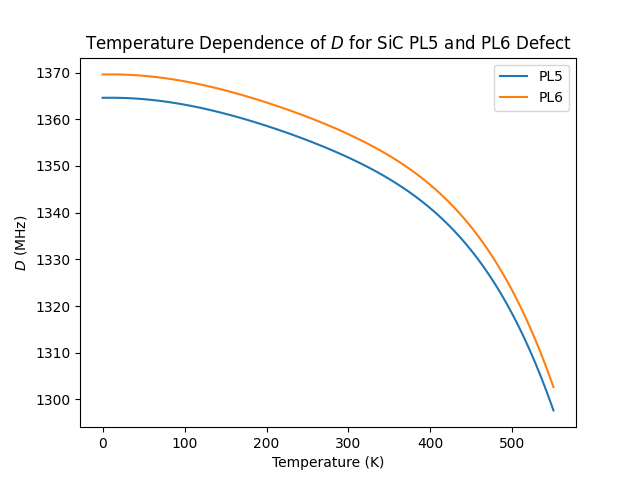
\includegraphics[width=0.49\textwidth]{figures/SiC-PL5PL6-D(T).png}
    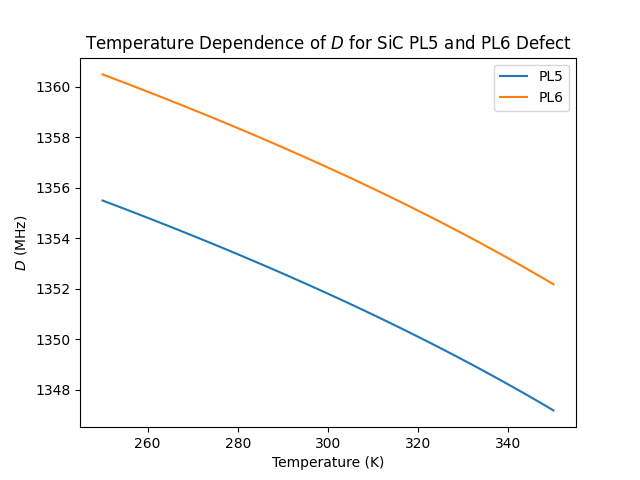
\includegraphics[width=0.49\textwidth]{figures/SiC-PL5PL6-D(T)-close.png}
    \caption{ZFS parameter $D$ temperature dependence for the PL5 and PL6 $S=1$ defect in SiC from 0-550 K (left) and 250-350 K (right). }\label{fig:PL5PL6DvsT}
\end{center}
\end{figure}

\td{Update the T dependence of PL5 and PL6 and regen the figure. Also update temp linear range in figure caption.}

In the simplest case thermometry is then achieved in the presence of a well known applied magnetic field. 

The measurement stems from the change of the value of
D mapped into the change of the oscillation frequency of the
relative variation of the photoluminescence intensity induced by the microwave pulse sequence.

Since the degeneracy is raised symmetrically, the value of $D$ is the average of the two resonant frequencies. The value of $D$ can then be mapped to a temperature. 

This is visualised in figure \ref{fig:pl6-3temps}. 

\begin{figure}[h]
    \begin{center}
        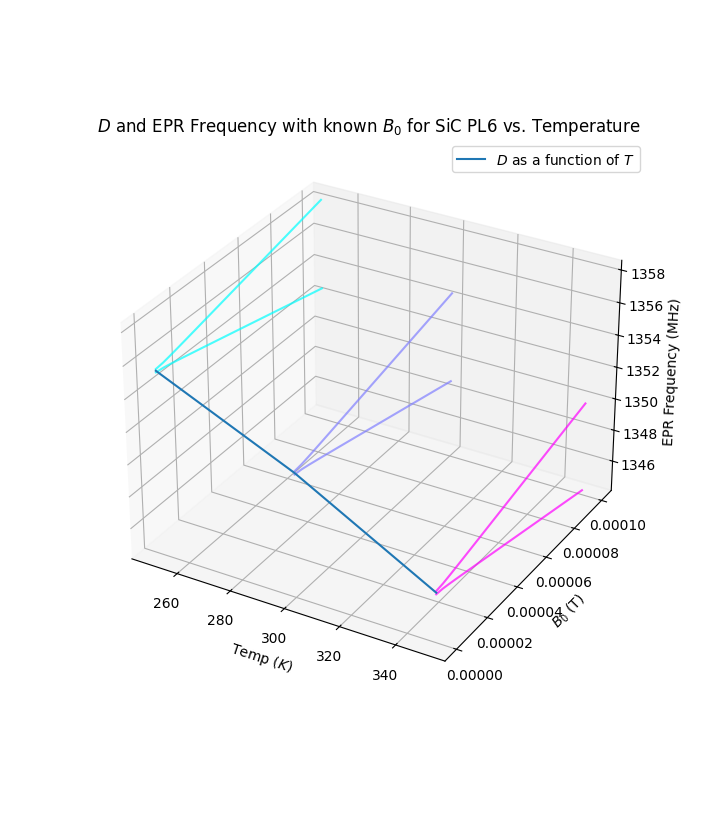
\includegraphics[width=0.8\textwidth]{figures/PL6-DvsT-3temps.png}
    \end{center}
    \caption{\td{write caption}}\label{fig:pl6-3temps}
\end{figure}

In practice this \td{Write up the Ramsey Interference methods for c-axis and basal from Castello p18}. 


